\chapter{Metodología}\label{cap3}

\section{Series de datos}

En la empresa de recambios de automóvil de estudio, las distintas referencias se agrupan en familias de productos para recibir un tratamiento común independientemente de la marca. Por ejemplo, todas las referencias únicas referidas a baterías pertenecen a la familia de baterías. Los datos que se obtienen del ERP son el agrupado de ventas diarias de cada familia de estudio. Las familias de producto utilizadas en este estudio son las siguientes:

\begin{itemize}
    \item Baterías.
    \item Filtros.
    \item Aceites.
    \item Limpiaparabrisas.
\end{itemize} 

En cuanto al rango de fechas de los datos se incluye desde el inicio de la empresa a mediados de 2008 hasta la mitad del año 2024. Para evitar el efecto del comienzo de la empresa y tomar los años completos, los datos se toman desde el 1 de enero de 2012 hasta el 31 de diciembre de 2023, dejando la primera mitad del año 2024 como test para los modelos. Además, como los días de apertura son de lunes a viernes, se excluyen los fines de semana para facilitar el trabajo a los modelos.

Los datos se encuentran en un archivo .csv y se cargan en Python en un \textit{DataFrame} de la librería Pandas \cite{pandas}. En el Código \ref{3-codcarga} se muestra un ejemplo de la carga de los datos de la familia de filtros. 

\lstinputlisting[caption=Carga de datos, label={3-codcarga}]{codigos/carga_datos.py}

A continuación, en la Tabla \ref{3-cabezafiltros} se observa una muestra con los cinco primeros datos como referencia de la estructura de los datos de las series.

\begin{table}[H]
	\ttabbox[\FBwidth]
	{\caption{Cabeza de la serie histórica de ventas de filtros}\label{3-cabezafiltros}}
	{\begin{tabular}{|P{3 cm}|P{4 cm}|}
		\hline
        \textbf{Fecha} & \textbf{Unidades vendidas} \\
        \hline
        2010-01-01 & 0 \\
        \hline
        2010-01-04 & 4 \\
        \hline
        2010-01-05 & 3 \\
        \hline
        2010-01-06 & 0 \\
        \hline
        2010-01-07 & 10 \\
        \hline
	\end{tabular}}
\end{table}


\subsection{Baterías}

Las baterías forman un grupo de producto el cual resulta relevante de estudio, ya que son un elemento común a todos los vehículos que se puede considerar consumible, ya que con el tiempo se degradan y es necesaria su sustitución. Además, son un elemento perecedero y por ello es necesario que pasen en el almacén el menor tiempo posible para evitar posibles fallos y, posteriores devoluciones por garatía. También hay que tener en cuenta que las baterías son productos más voluminosos y pesados, por lo que el coste de inventario es superior a la media de los demás productos.

En la Figura \ref{3-graf_baterias}, se observa una gráfica de la serie temporal, donde se muestra una clara tendencia al alza y cierta estacionalidad. Además, a destacar el bajón de ventas producidas por el confinamiento durante el COVID y el posterior incremento de las ventas al ser diferidas.

\begin{figure}[H]
	\ffigbox[\FBwidth] {
	\caption{Gráfica de la serie temporal de ventas de baterías}\label{3-graf_baterias}
	}
	{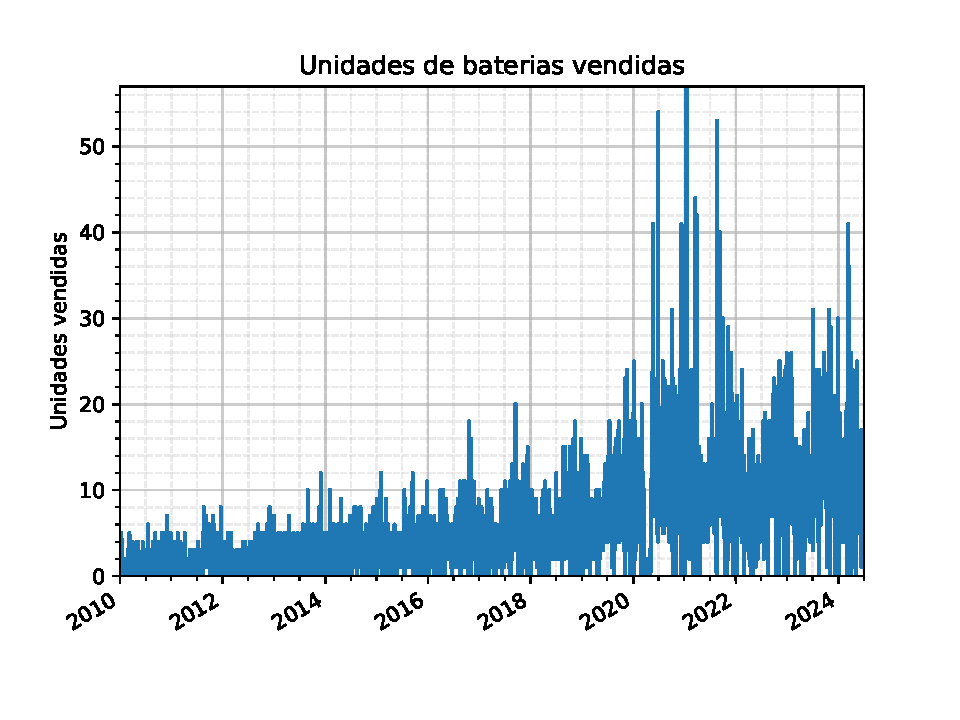
\includegraphics[width=0.75\textwidth]{imagenes/grafica_baterias.pdf}}
\end{figure}

Utilizando la librería Prophet \cite{prophet}, se desglosa la estacionalidad de la serie temporal, mostrada en la Figura \ref{3-comp_baterias}. La primera subgráfica muestra la tendencia al alza en las ventas de esta familia. La segunda, muestra la estacionalidad intrasemanal, donde muestra que la mayoría de ventas se producen a comienzo de semana. En la última, la estacionalidad anual muestra que las ventas entorno al mes de abril son las más bajas del año, mientras que a partir de septiembre se incrementan considerablemente.

\begin{figure}[H]
	\ffigbox[\FBwidth] {
	\caption{Gráfica de componentes de la serie de baterías}\label{3-comp_baterias}
	}
	{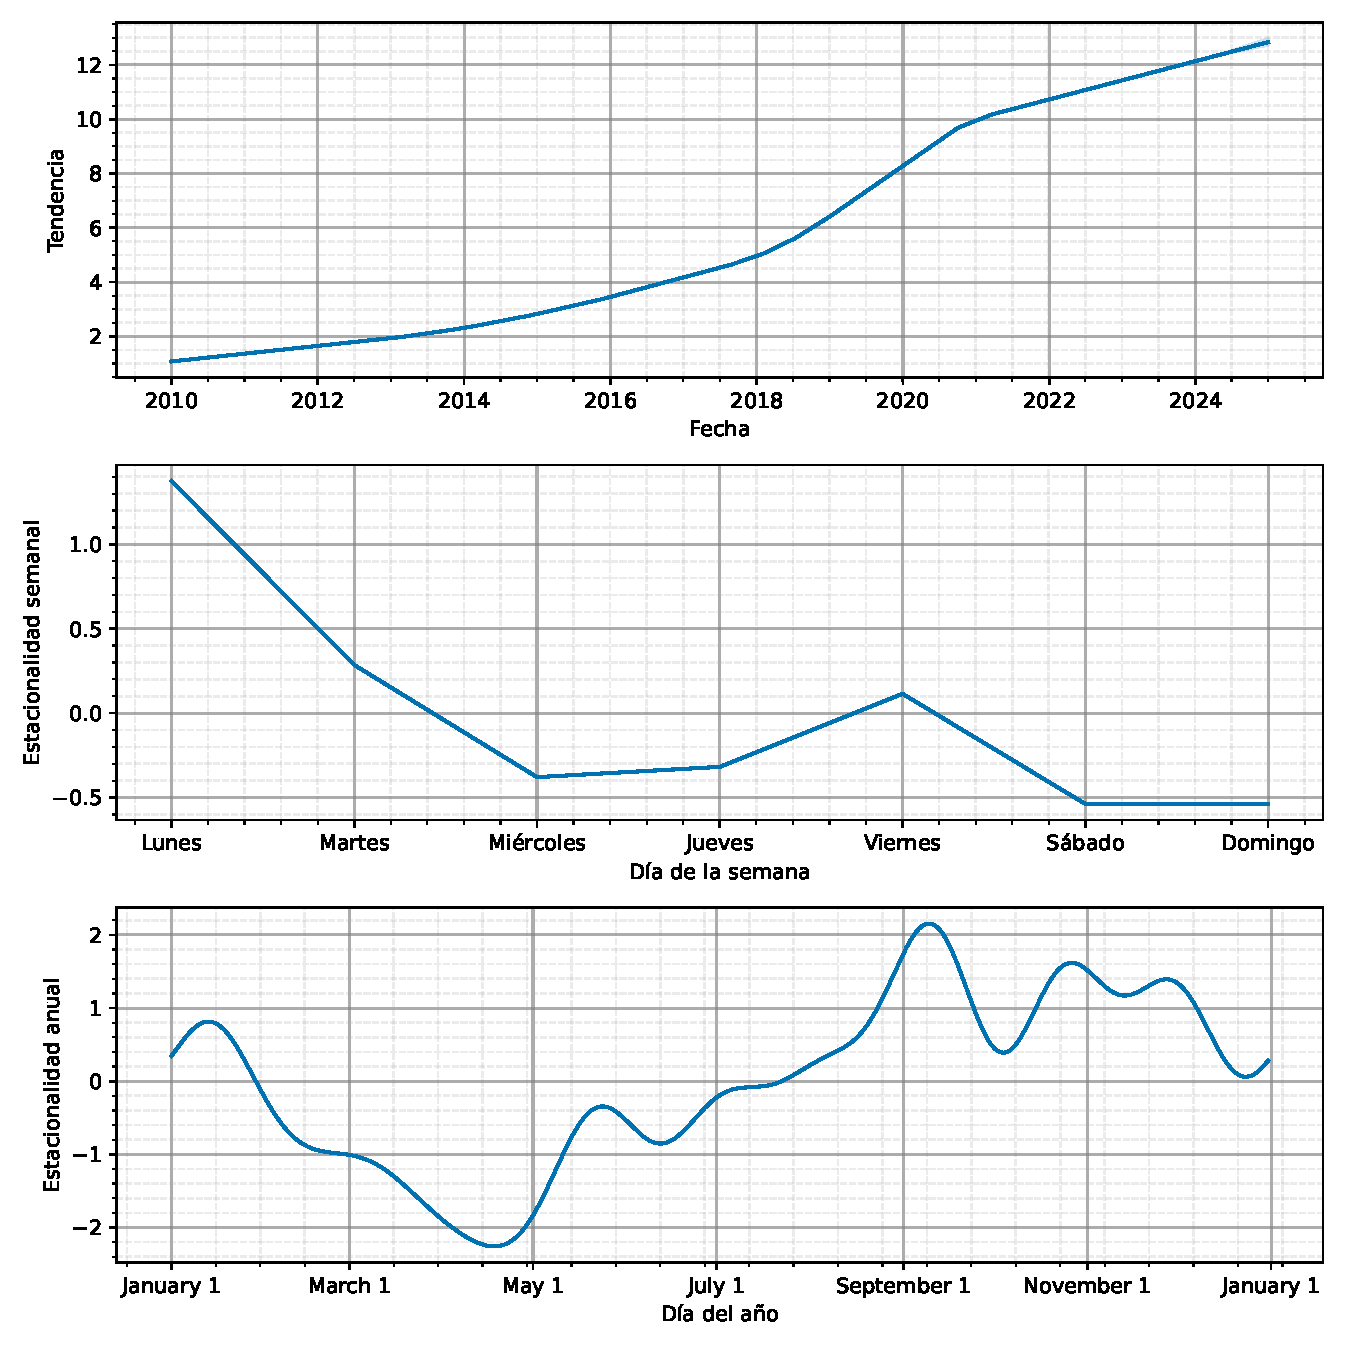
\includegraphics[width=0.75\textwidth]{imagenes/comps_baterias.pdf}}
\end{figure}


\subsection{Filtros}

Los filtros son el consumible por excelencia de los vehículos con motores de combustión, ya que la sustitución periódica de filtros como el de aceite y el de combustible es esencial para alargar la vida útil del motor. Además, también hay filtros como el de aire que se encuentran también en vehículos eléctricos. Por esto, se conforma una familia de producto que tiene un alto volumen de ventas.

En la Figura \ref{3-graf_filtros} se observa el histórico de datos de la familia de producto. No se aprecia tanta estacionalidad como en el caso de las baterías, pero la tendencia al alza es bastante clara en los primeros años, con un estancamiento a partir del año 2020.

\begin{figure}[H]
	\ffigbox[\FBwidth] {
	\caption{Gráfica de la serie temporal de ventas de baterías}\label{3-graf_filtros}
	}
	{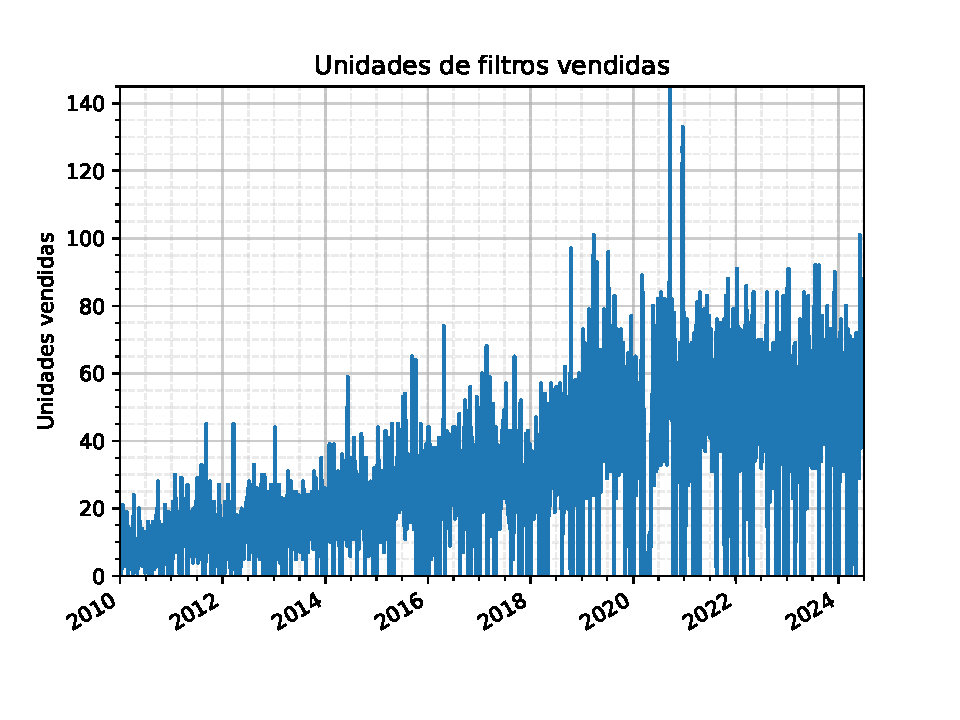
\includegraphics[width=0.75\textwidth]{imagenes/grafica_filtros.pdf}}
\end{figure}

Desglosando los componentes estacionales, no se observa una estacionalidad muy marcada a nivel semanal, pero sí a nivel anual, donde la mayoría de mantenimientos se realizan previos a períodos vacacionales.

\begin{figure}[H]
	\ffigbox[\FBwidth] {
	\caption{Gráfica de componentes}\label{3-comp_filtros}
	}
	{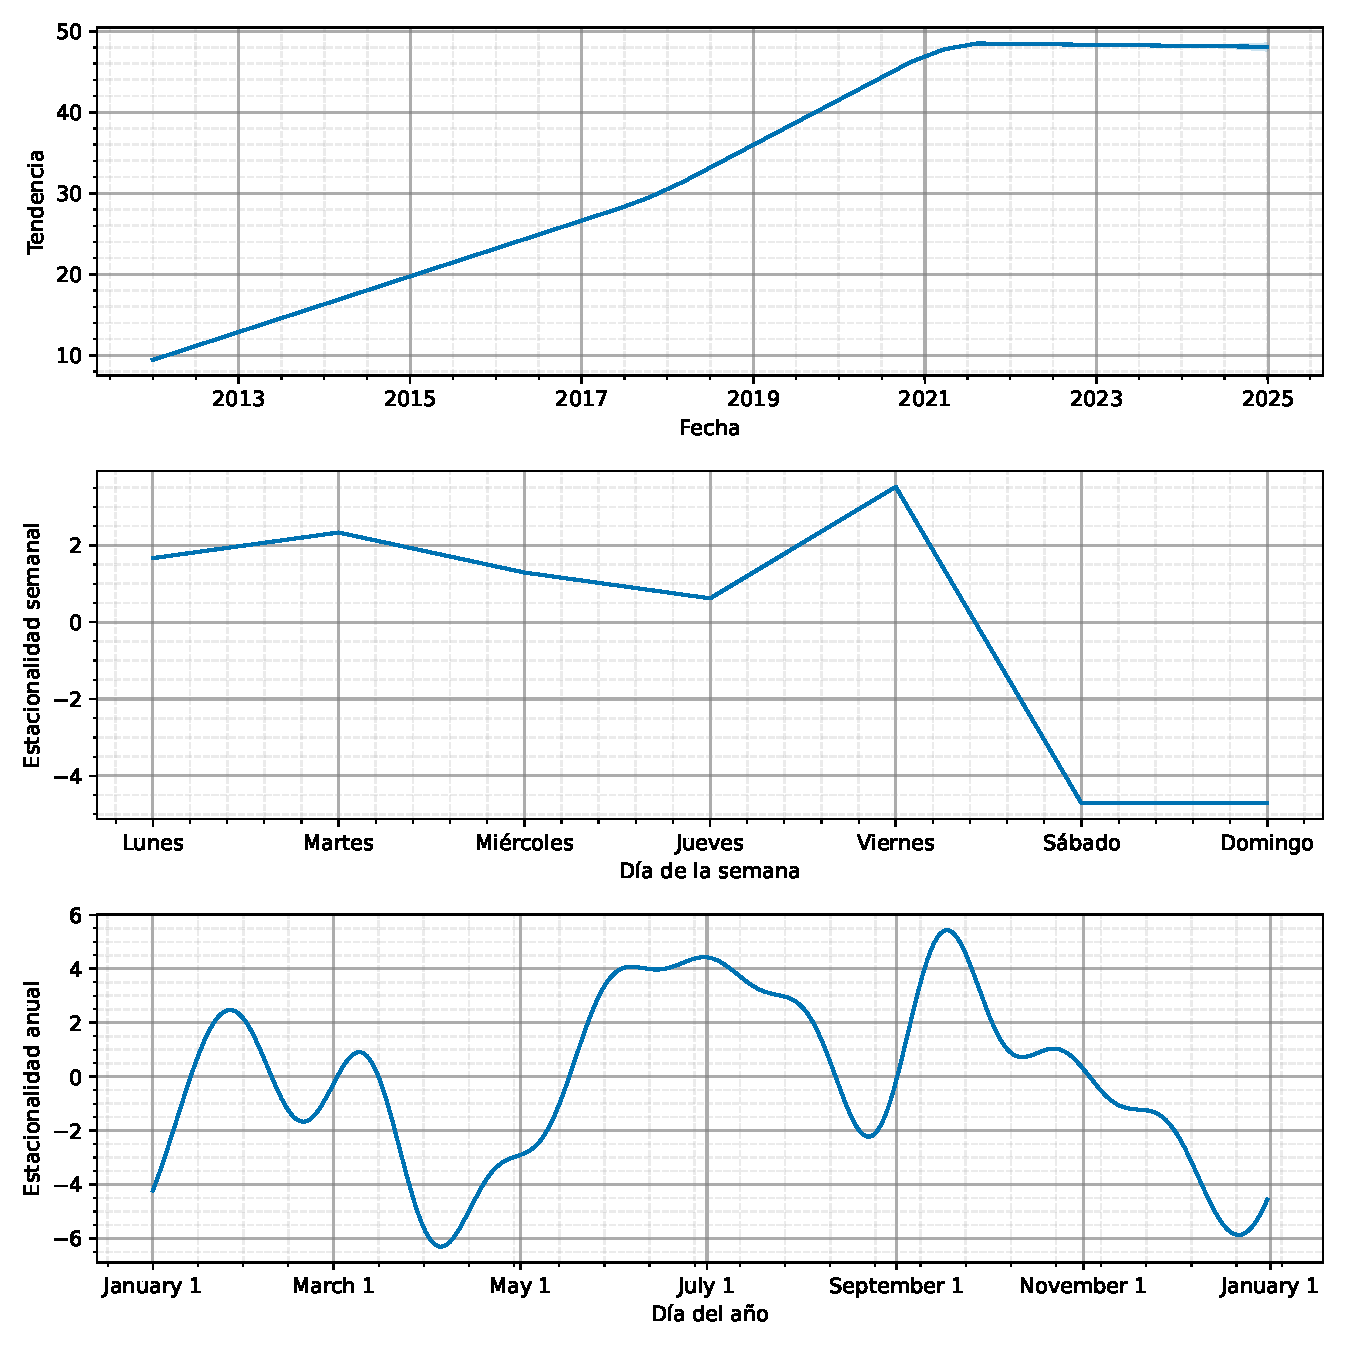
\includegraphics[width=0.75\textwidth]{imagenes/comps_filtros.pdf}}
\end{figure}

\subsection{Aceites}

\begin{figure}[H]
	\ffigbox[\FBwidth] {
	\caption{Gráfica de la serie temporal de ventas de aceites}\label{3-graf_aceites}
	}
	{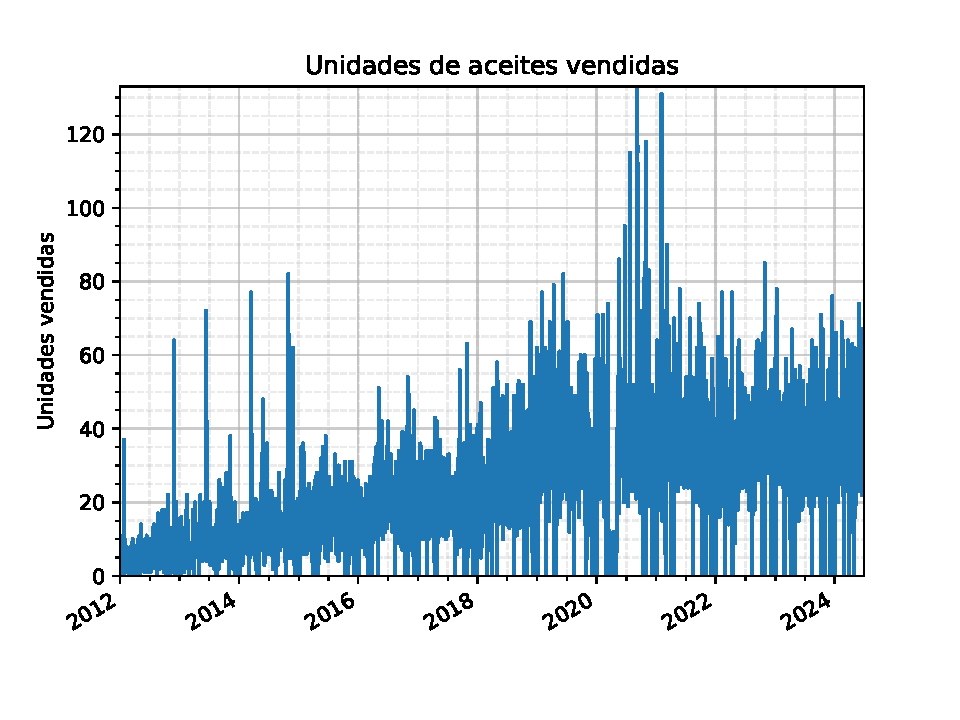
\includegraphics[width=0.75\textwidth]{imagenes/grafica_aceites.pdf}}
\end{figure}

\begin{figure}[H]
	\ffigbox[\FBwidth] {
	\caption{Gráfica de componentes}\label{3-comp_aceites}
	}
	{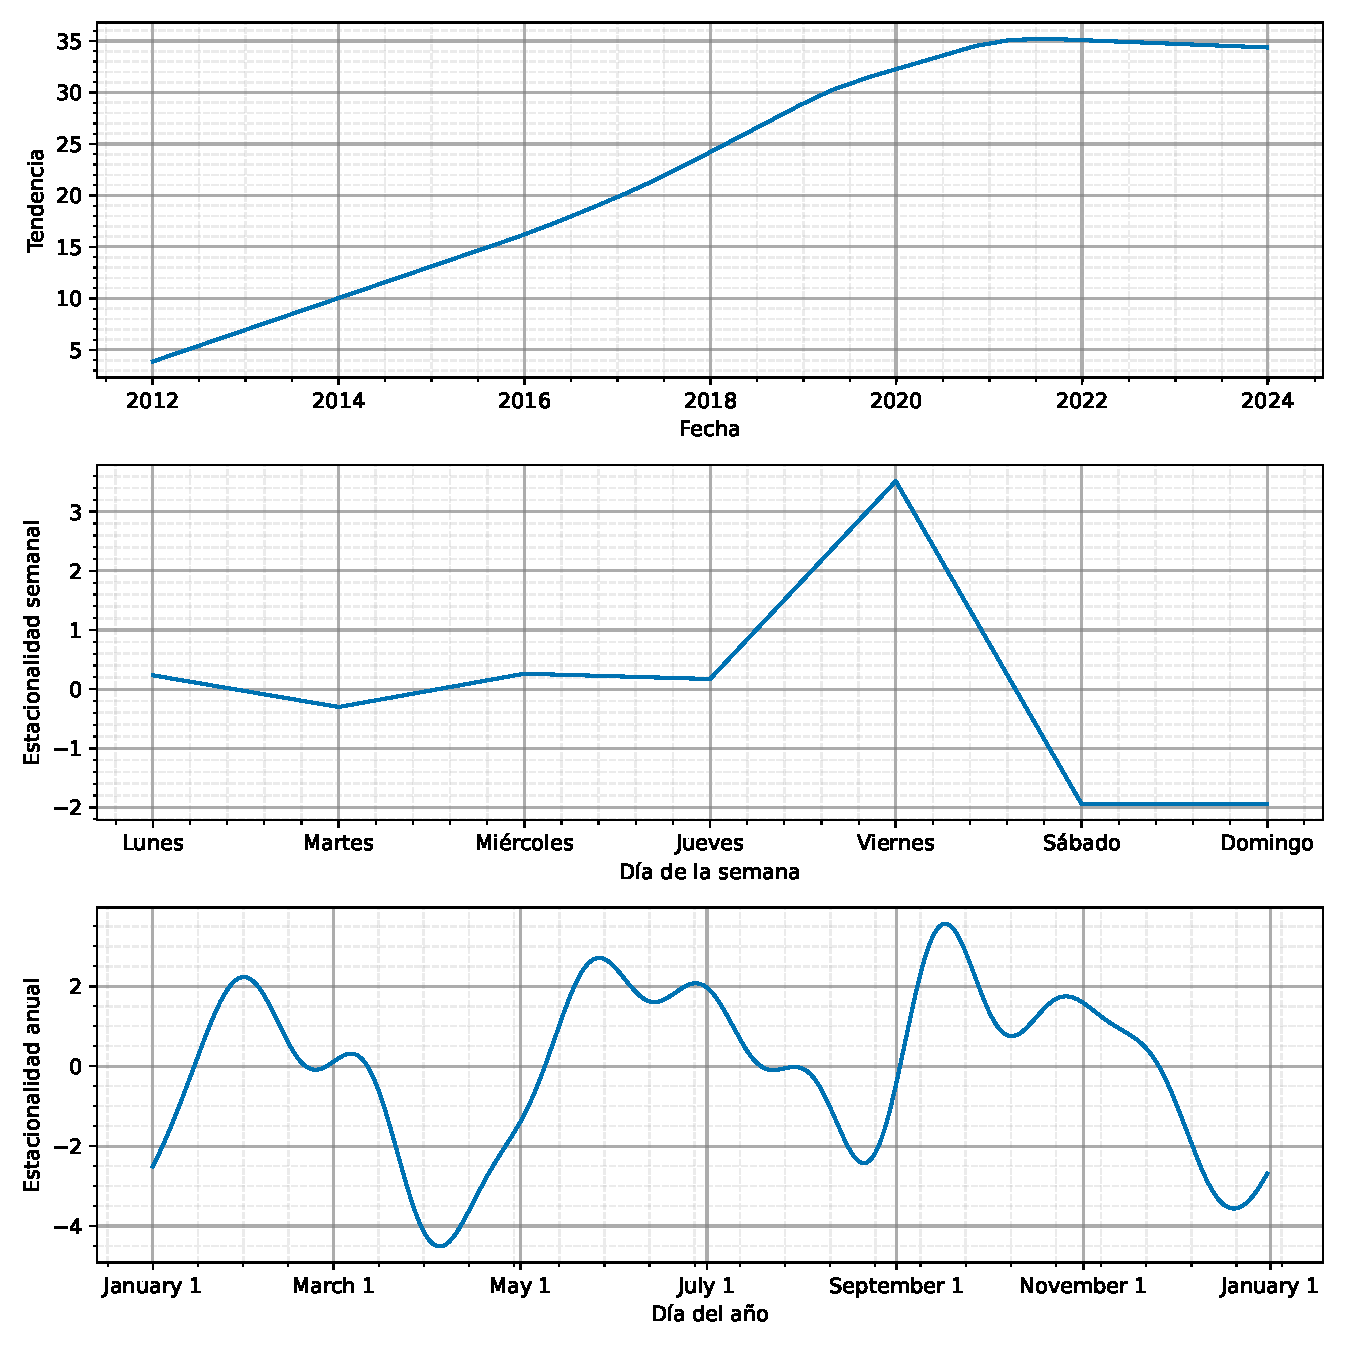
\includegraphics[width=0.75\textwidth]{imagenes/comps_aceites.pdf}}
\end{figure}

\subsection{Limpiaparabrisas}

\begin{figure}[H]
	\ffigbox[\FBwidth] {
	\caption{Gráfica de la serie temporal de ventas de limpiaparabrisas}\label{3-graf_limpiaparabrisas}
	}
	{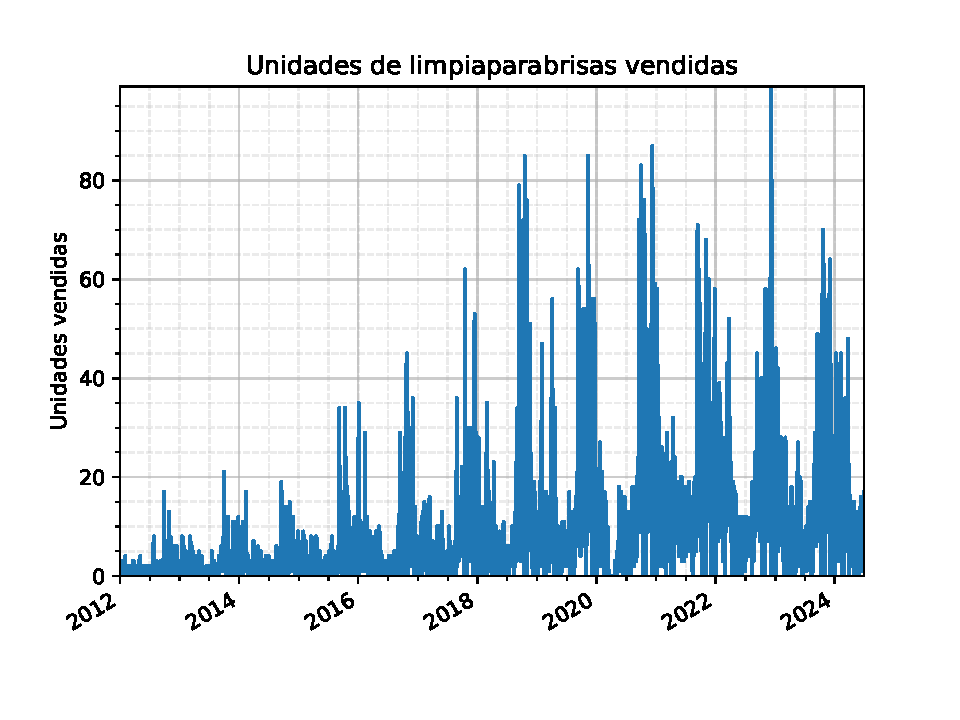
\includegraphics[width=0.75\textwidth]{imagenes/grafica_limpiaparabrisas.pdf}}
\end{figure}

\begin{figure}[H]
	\ffigbox[\FBwidth] {
	\caption{Gráfica de componentes}\label{3-comp_limpiaparabrisas}
	}
	{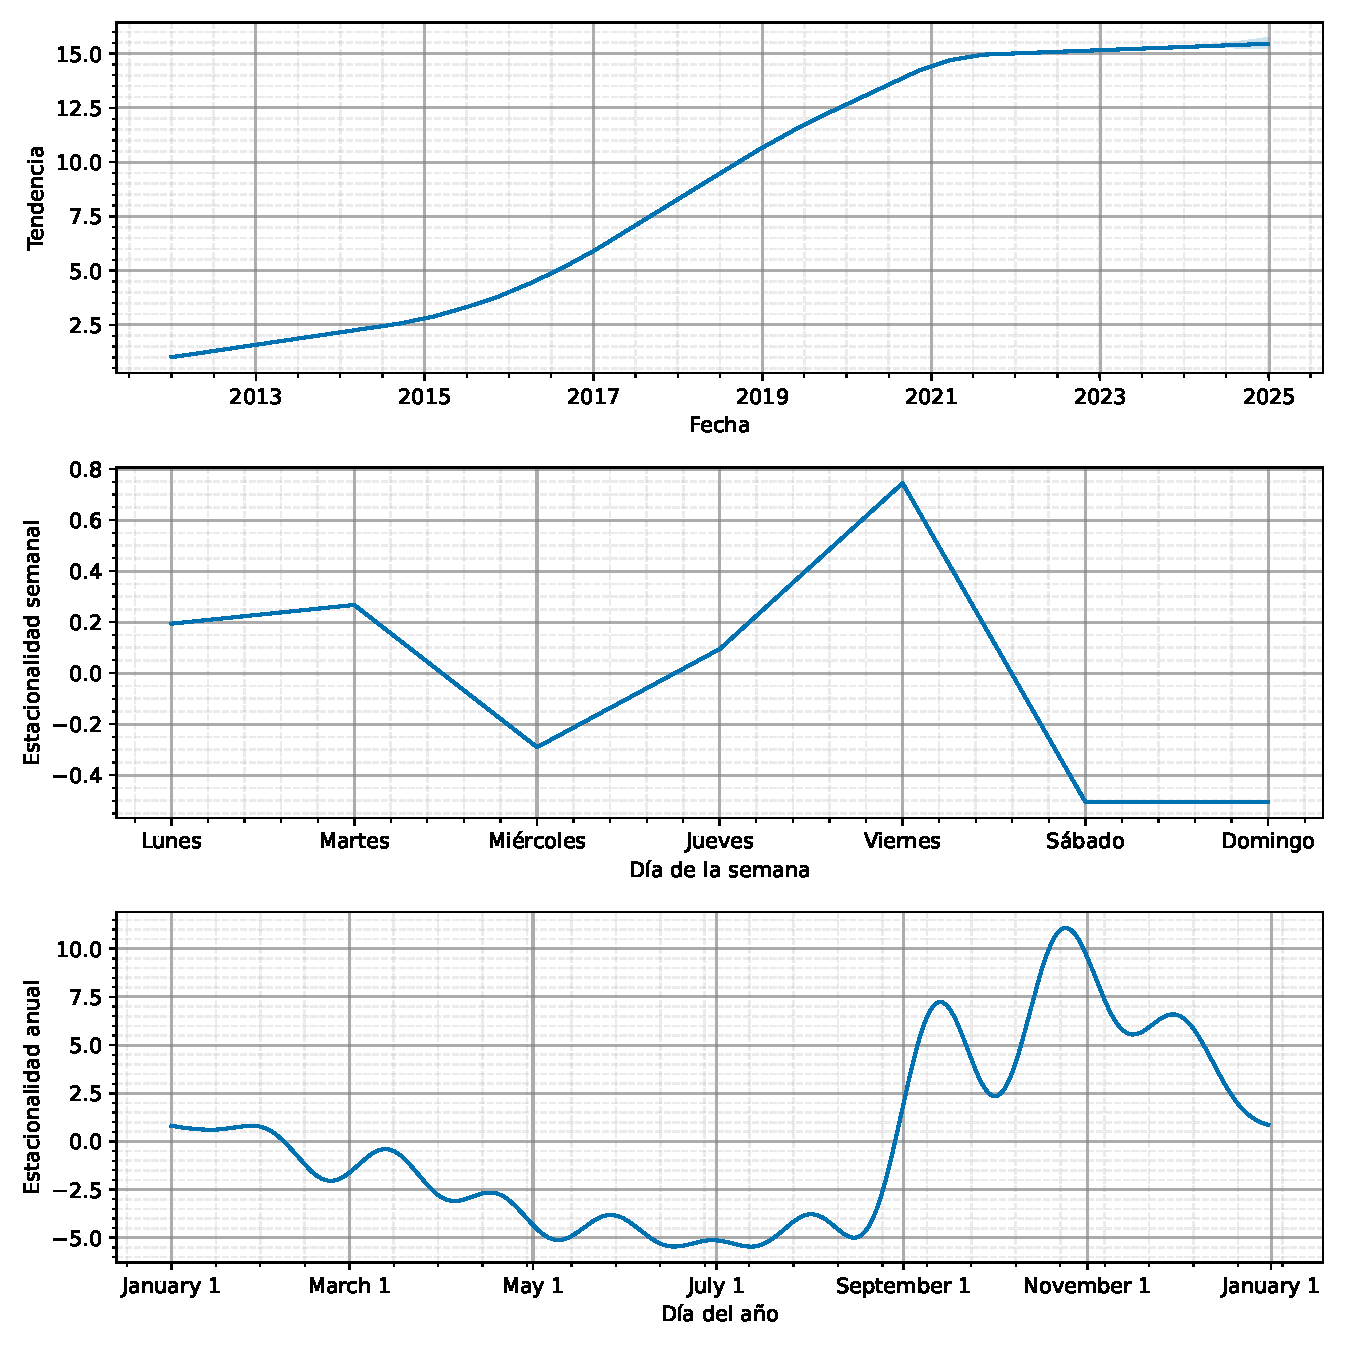
\includegraphics[width=0.75\textwidth]{imagenes/comps_limpiaparabrisas.pdf}}
\end{figure}